\documentclass[aspectratio=169,11pt]{beamer}

\usepackage[T1]{fontenc}
\usepackage[utf8]{inputenc}
\usepackage[brazilian]{babel}
\usepackage{lmodern}
\usepackage{graphicx}
\usepackage{booktabs}
\usepackage{amsmath}
\usepackage{pgfplots}
\usepackage{pgfplotstable}
\pgfplotsset{compat=1.18}
\usepackage{hyperref}
\usepackage{multicol}
\usepackage{tikz}

% -----------------------------------------------------------------------------
% Identidade visual
% -----------------------------------------------------------------------------
\definecolor{RoxoPrincipal}{HTML}{4D4057}
\definecolor{RoxoSecundario}{HTML}{75657F}
\definecolor{MalvaDestaque}{HTML}{9A6F86}
\definecolor{LavandaClaro}{HTML}{F1EDF3}
\definecolor{LavandaLinha}{HTML}{D8CFDD}
\definecolor{CinzaTexto}{HTML}{413C43}

\usetheme{default}
\useinnertheme{rounded}
\setbeamertemplate{navigation symbols}{}

\setbeamercolor{normal text}{fg=CinzaTexto,bg=white}
\setbeamercolor{structure}{fg=RoxoPrincipal}
\setbeamercolor{title}{fg=white}
\setbeamercolor{subtitle}{fg=white}
\setbeamercolor{author}{fg=white}
\setbeamercolor{institute}{fg=white!90}
\setbeamercolor{date}{fg=white!80}
\setbeamercolor{frametitle}{fg=white,bg=RoxoPrincipal}
\setbeamercolor{block title}{fg=white,bg=RoxoSecundario}
\setbeamercolor{block body}{fg=CinzaTexto,bg=LavandaClaro}
\setbeamercolor{block title alerted}{fg=white,bg=MalvaDestaque}
\setbeamercolor{block body alerted}{fg=CinzaTexto,bg=LavandaClaro}
\setbeamercolor{alerted text}{fg=MalvaDestaque}
\setbeamercolor{footline}{fg=RoxoPrincipal,bg=white}
\setbeamercolor{footline line}{bg=LavandaLinha}

\setbeamerfont{title}{size=\LARGE,series=\bfseries}
\setbeamerfont{subtitle}{size=\large}
\setbeamerfont{frametitle}{size=\large,series=\bfseries}
\setbeamerfont{footline}{size=\scriptsize}

% Logo da UFPE com uma base clara para contraste.
\newcommand{\marcaInstitucional}[1]{%
  \begin{tikzpicture}[baseline=(marca.base)]
    \node[fill=white,rounded corners=2pt,inner sep=2.2pt] (marca) {%
      
\includegraphics[height=#1]{logo_ufpe.png}%
    };
  \end{tikzpicture}%
}

% Cabeçalho roxo com a marca institucional em todos os slides de conteúdo.
\setbeamertemplate{frametitle}{%
  \nointerlineskip
  \begin{beamercolorbox}[
    wd=\paperwidth,ht=3.4ex,dp=1.45ex,leftskip=0.58cm,rightskip=1.75cm
  ]{frametitle}%
    \usebeamerfont{frametitle}\insertframetitle
  \end{beamercolorbox}%
  \begin{tikzpicture}[remember picture,overlay]
    \node[anchor=north east,fill=white,rounded corners=2pt,inner sep=1.2pt]
      at ([xshift=-0.32cm,yshift=-0.16cm]current page.north east)
      {
\includegraphics[height=0.52cm]{logo_ufpe.png}};
  \end{tikzpicture}%
}

% Rodapé leve, com seção atual e paginação em formato de cápsula.
\setbeamertemplate{footline}{%
  \leavevmode%
  \vbox{%
    \begin{beamercolorbox}[wd=\paperwidth,ht=0.22ex,dp=0ex]{footline line}
    \end{beamercolorbox}%
    \hbox{%
      \begin{beamercolorbox}[wd=.28\paperwidth,ht=3.0ex,dp=1.15ex,leftskip=0.55cm]{footline}
        \usebeamerfont{footline}\insertshortauthor
      \end{beamercolorbox}%
      \begin{beamercolorbox}[wd=.52\paperwidth,ht=3.0ex,dp=1.15ex,center]{footline}
        \usebeamerfont{footline}\insertsectionhead
      \end{beamercolorbox}%
      \begin{beamercolorbox}[wd=.20\paperwidth,ht=3.0ex,dp=0.65ex,rightskip=0.45cm plus 1fil]{footline}
        \tikz[baseline=-0.65ex]{%
          \node[fill=RoxoPrincipal,text=white,rounded corners=5pt,
            inner xsep=7pt,inner ysep=2.3pt] {%
            \usebeamerfont{footline}\insertframenumber\,/\,\inserttotalframenumber
          };
        }%
      \end{beamercolorbox}%
    }%
  }%
  \vskip0pt%
}

% -----------------------------------------------------------------------------
% Informações editáveis da apresentação
% -----------------------------------------------------------------------------
\newcommand{\telefone}{(81) 98538-4702}
\newcommand{\email}{Romadeoliveira@hotmail.com}
\newcommand{\linkedin}{linkedin.com/in/romariojonas-veloso-427373175}
\newcommand{\portfolio}{romariojonas.com}
\newcommand{\lattes}{lattes.cnpq.br/7040983804231610}

\title[Filtro RC e efeito de carga]{Filtro RC Passa-Baixa e Efeito de Carga}
\subtitle{Projeto, resposta em frequência e isolamento da carga com buffer}
\author[Romário J. O. Veloso]{Romário J. O. Veloso}
\institute{Bacharelando em Engenharia Eletrônica\\
Universidade Federal de Pernambuco -- UFPE\\
Centro de Tecnologia e Geociências -- CTG\\
Departamento de Eletrônica e Sistemas -- DES}
\date{Prática 4 -- Circuitos Elétricos 2 -- 2026.2}

\pgfplotsset{
  grafico/.style={
    width=\linewidth,
    height=0.49\textheight,
    grid=both,
    major grid style={LavandaLinha},
    minor grid style={LavandaClaro},
    tick label style={font=\scriptsize},
    label style={font=\scriptsize},
    legend style={font=\scriptsize,draw=none,fill=white},
    scaled ticks=false,
  }
}

\begin{document}

{
\setbeamercolor{background canvas}{bg=RoxoPrincipal}
\setbeamertemplate{footline}{}
\begin{frame}[plain]
  \begin{center}
    \vspace{0.06cm}
    \marcaInstitucional{1.30cm}\par
    \vspace{0.28cm}
    {\usebeamerfont{title}\color{white}\inserttitle\par}
    \vspace{0.18cm}
    {\usebeamerfont{subtitle}\color{white!82}\insertsubtitle\par}
    \vspace{0.26cm}
    {\color{MalvaDestaque}\rule{0.22\textwidth}{2pt}}\par
    \vspace{0.26cm}
    {\usebeamerfont{author}\color{white}\insertauthor\par}
    \vspace{0.10cm}
    {\usebeamerfont{institute}\color{white!84}\insertinstitute\par}
    \vfill
    {\color{white!72}\small\insertdate\quad\textbullet\quad Recife -- Pernambuco}
  \end{center}
\end{frame}
}

\begin{frame}{Sumário}
  \tableofcontents[hideallsubsections]
\end{frame}


\section{Introdução}
\begin{frame}{Contexto da prática}
  \begin{block}{Problema investigado}
    Um filtro RC mantém sua resposta quando uma carga é conectada à saída?
    Como um amplificador operacional pode reduzir a influência dessa carga?
  \end{block}

  \begin{columns}[T,onlytextwidth]
    \begin{column}{0.48\textwidth}
      \textbf{Grandezas observadas}
      \begin{itemize}
        \item ganho em baixas frequências;
        \item frequência de corte;
        \item magnitude de $H(j\omega)$;
        \item atenuação das altas frequências.
      \end{itemize}
    \end{column}
    \begin{column}{0.48\textwidth}
      \textbf{Três condições de operação}
      \begin{itemize}
        \item filtro RC sem carga;
        \item carga resistiva ligada diretamente;
        \item carga isolada por um buffer.
      \end{itemize}
    \end{column}
  \end{columns}
\end{frame}

\begin{frame}{Objetivos}
  \begin{block}{Objetivo geral}
    Projetar e analisar um filtro RC passa-baixa de primeira ordem, verificando
    o efeito de carga e a atuação de um seguidor de tensão na resposta em frequência.
  \end{block}

  \begin{itemize}
    \item Deduzir $H_1(s)$, $H_2(s)$ e $H_3(s)$ a partir das equações dos circuitos.
    \item Dimensionar um filtro com ganho unitário e corte de $50\,\mathrm{Hz}$.
    \item Comparar ganho e frequência de corte com e sem carga.
    \item Validar as respostas por diagramas de Bode e simulação no LTspice.
    \item Recalcular os modelos com os componentes medidos e comparar com a bancada.
  \end{itemize}
\end{frame}

\begin{frame}{Metodologia de validação}
  \small
  \begin{columns}[T,onlytextwidth]
    \begin{column}{0.31\textwidth}
      \begin{block}{1. Análise teórica}
        \begin{itemize}
          \item impedância $Z_C=1/(sC)$;
          \item aplicação da lei das correntes;
          \item resolução simbólica;
          \item projeto e diagramas de Bode.
        \end{itemize}
      \end{block}
    \end{column}
    \begin{column}{0.31\textwidth}
      \begin{block}{2. Simulação}
        \begin{itemize}
          \item três configurações no LTspice;
          \item fonte AC unitária;
          \item varredura logarítmica;
          \item buffer alimentado em $\pm10\,\mathrm{V}$.
        \end{itemize}
      \end{block}
    \end{column}
    \begin{column}{0.31\textwidth}
      \begin{block}{3. Ensaio em bancada}
        \begin{itemize}
          \item aferição dos componentes;
          \item montagem em protoboard;
          \item medição de $V_i$ e $V_o$;
          \item cálculo de $|H|=V_o/V_i$.
        \end{itemize}
      \end{block}
    \end{column}
  \end{columns}

  \begin{alertblock}{Condição de comparação}
    A tensão de entrada é medida em cada frequência.
    O corte corresponde a uma queda de $3\,\mathrm{dB}$ em relação ao ganho
    de baixa frequência de cada configuração.
  \end{alertblock}
\end{frame}

\begin{frame}{Três configurações do filtro RC}
  \begin{columns}[T,onlytextwidth]
    \begin{column}{0.31\textwidth}
      \centering
      \textbf{1. Sem carga}

      \vspace{0.16cm}
      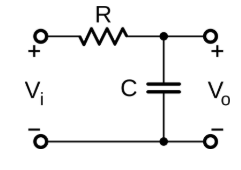
\includegraphics[width=\linewidth,height=0.31\textheight,keepaspectratio]{slides/img/circuito_1.png}

      \begin{block}{Referência}
        \small Saída medida sobre o capacitor, sem uma carga resistiva adicional.
      \end{block}
    \end{column}
    \begin{column}{0.31\textwidth}
      \centering
      \textbf{2. Com carga direta}

      \vspace{0.16cm}
      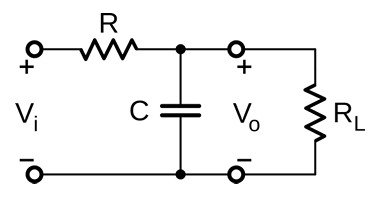
\includegraphics[width=\linewidth,height=0.31\textheight,keepaspectratio]{slides/img/circuito_2.png}

      \begin{block}{Efeito de carga}
        \small $R_L$ fica em paralelo com $C$, alterando o ganho e a constante de tempo.
      \end{block}
    \end{column}
    \begin{column}{0.31\textwidth}
      \centering
      \textbf{3. Com buffer}

      \vspace{0.16cm}
      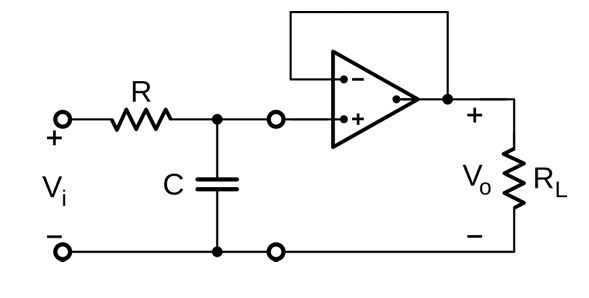
\includegraphics[width=\linewidth,height=0.31\textheight,keepaspectratio]{slides/img/circuito_3.png}

      \begin{block}{Isolamento}
        \small O seguidor de tensão fornece corrente à carga sem carregar o nó RC ideal.
      \end{block}
    \end{column}
  \end{columns}
\end{frame}


\section{Análise teórica}
\begin{frame}{Circuito 1: modelagem sem carga}
  \small
  \begin{columns}[T,onlytextwidth]
    \begin{column}{0.46\textwidth}
      \centering
      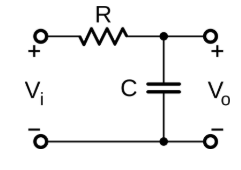
\includegraphics[width=0.65\linewidth,height=0.28\textheight,keepaspectratio]{slides/img/circuito_1.png}

      \begin{block}{Equação no domínio de Laplace}
        Com condições iniciais nulas,
        \[
          \frac{V_i-V_o}{R}=sCV_o.
        \]
        A saída é a tensão sobre o capacitor.
      \end{block}
    \end{column}
    \begin{column}{0.50\textwidth}
      \begin{alertblock}{Função de transferência}
        \[
          H_1(s)=\frac{V_o}{V_i}
          =\frac{Z_C}{R+Z_C}
          =\frac{1}{1+sRC}.
        \]
        \[
          K_1=H_1(0)=1,\qquad \tau_1=RC.
        \]
        \[
          p_1=-\frac{1}{RC},\qquad
          f_{c1}=\frac{1}{2\pi RC}.
        \]
      \end{alertblock}
      Em baixas frequências, $|H_1|\approx1$.
      Em altas frequências, a saída é atenuada.
    \end{column}
  \end{columns}
  \vspace{0.12cm}
  \centering\scriptsize
  Para uma fonte com resistência série $R_s$, o modelo referido à fonte ideal usa $R+R_s$.
  Nas medições, $V_i$ é obtido na entrada do filtro.
\end{frame}

\begin{frame}{Projeto para frequência de corte de 50 Hz}
  \begin{columns}[T,onlytextwidth]
    \begin{column}{0.48\textwidth}
      \begin{block}{Especificação do roteiro}
        Ganho unitário, $f_c=50\,\mathrm{Hz}$ e $C=100\,\mathrm{nF}$.
        \[
          R=\frac{1}{2\pi f_c C}
          \approx31{,}83\,\mathrm{k}\Omega.
        \]
        Escolha comercial:
        \[
          \boxed{R=33\,\mathrm{k}\Omega}.
        \]
      \end{block}
    \end{column}
    \begin{column}{0.48\textwidth}
      \begin{alertblock}{Resposta com o valor comercial}
        \[
          \tau=3{,}3\,\mathrm{ms},\qquad K=1.
        \]
        \[
          H_1(s)=\frac{1}{1+0{,}0033s}.
        \]
        \[
          f_c\approx48{,}23\,\mathrm{Hz}.
        \]
        O ajuste do resistor desloca o corte em aproximadamente $-3{,}54\%$.
      \end{alertblock}
    \end{column}
  \end{columns}

  \vspace{0.10cm}
  \centering\scriptsize
  Projeto nominal: $R=33\,\mathrm{k}\Omega$, $C=100\,\mathrm{nF}$ e, quando presente,
  $R_L=22\,\mathrm{k}\Omega$. A bancada será comparada com seus próprios componentes medidos.
\end{frame}

\begin{frame}{Circuito 2: efeito da carga resistiva}
  \small
  \begin{columns}[T,onlytextwidth]
    \begin{column}{0.47\textwidth}
      \begin{block}{Equação nodal e função de transferência}
        \[
          \frac{V_i-V_o}{R}=sCV_o+\frac{V_o}{R_L}.
        \]
        \[
          H_2(s)=\frac{R_L}{R+R_L+sCRR_L}
          =\frac{K_2}{1+s\tau_2}.
        \]
        \[
          K_2=\frac{R_L}{R+R_L},\qquad
          \tau_2=(R\parallel R_L)C.
        \]
      \end{block}
    \end{column}
    \begin{column}{0.49\textwidth}
      \begin{alertblock}{Projeto nominal com carga de $22\,\mathrm{k}\Omega$}
        \[
          R\parallel R_L=13{,}2\,\mathrm{k}\Omega.
        \]
        \[
          K_2=0{,}4\quad(-7{,}96\,\mathrm{dB}).
        \]
        \[
          f_{c2}=\frac{1}{2\pi(R\parallel R_L)C}
          \approx120{,}57\,\mathrm{Hz}.
        \]
        O ganho diminui, mas a frequência de corte aumenta:
        o capacitor passa a enxergar uma resistência equivalente menor.
      \end{alertblock}
    \end{column}
  \end{columns}
\end{frame}

\begin{frame}{Circuito 3: isolamento da carga com buffer}
  \small
  \begin{columns}[T,onlytextwidth]
    \begin{column}{0.48\textwidth}
      \centering
      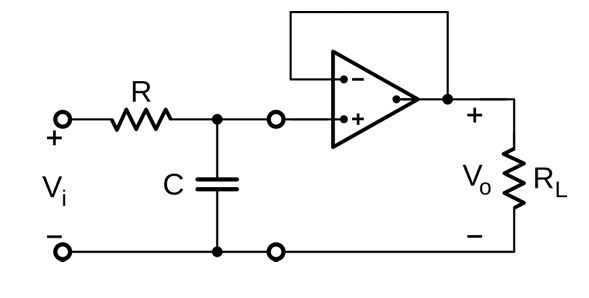
\includegraphics[width=\linewidth,height=0.27\textheight,keepaspectratio]{slides/img/circuito_3.png}

      \begin{block}{Modelo ideal do seguidor}
        $i^+=i^-=0$ e $v^-=v^+$.
        Como $v^-=V_o$, resulta $V_o=v^+$.
        \[
          \frac{V_i-v^+}{R}=sCv^+.
        \]
      \end{block}
    \end{column}
    \begin{column}{0.48\textwidth}
      \begin{alertblock}{Função de transferência restaurada}
        \[
          H_3(s)=\frac{1}{1+sRC}=H_1(s).
        \]
        \[
          K_3=1,\qquad f_{c3}=\frac{1}{2\pi RC}.
        \]
        No projeto nominal, $f_{c3}\approx48{,}23\,\mathrm{Hz}$.
        O valor de $R_L$ não entra na função de transferência ideal.
      \end{alertblock}
      A alimentação do ampop fornece a corrente de carga.
      O ganho de tensão do buffer é unitário.
    \end{column}
  \end{columns}
\end{frame}

\begin{frame}{Resposta nominal em frequência}
  \begin{columns}[c,onlytextwidth]
    \begin{column}{0.48\textwidth}
      \centering
      \begin{tikzpicture}
        \begin{semilogxaxis}[
          grafico,width=0.96\linewidth,xmin=0.01,xmax=100000,ymin=-70,ymax=3,
          xlabel={Frequência (Hz)},ylabel={Magnitude (dB)},legend pos=south west
        ]
          \addplot[very thick,RoxoPrincipal] table[x=f,y=ganho1_db]{slides/dados/resposta_nominal.dat};
          \addlegendentry{Sem carga = buffer ideal}
          \addplot[very thick,MalvaDestaque,dashed] table[x=f,y=ganho2_db]{slides/dados/resposta_nominal.dat};
          \addlegendentry{Carga direta}
        \end{semilogxaxis}
      \end{tikzpicture}
    \end{column}
    \begin{column}{0.48\textwidth}
      \centering
      \begin{tikzpicture}
        \begin{semilogxaxis}[
          grafico,width=0.96\linewidth,xmin=0.01,xmax=100000,ymin=-95,ymax=5,ytick={-90,-60,-30,0},
          xlabel={Frequência (Hz)},ylabel={Fase (graus)}
        ]
          \addplot[very thick,RoxoPrincipal] table[x=f,y=fase1_deg]{slides/dados/resposta_nominal.dat};
          \addplot[very thick,MalvaDestaque,dashed] table[x=f,y=fase2_deg]{slides/dados/resposta_nominal.dat};
        \end{semilogxaxis}
      \end{tikzpicture}
    \end{column}
  \end{columns}

  \small
  \begin{block}{Leitura dos diagramas}
    Sistemas de primeira ordem: queda assintótica de $20\,\mathrm{dB}$ por década
    e fase de $0^\circ$ a $-90^\circ$.
    O buffer ideal recupera a curva do filtro sem carga.
  \end{block}
  \centering\scriptsize
  $R=33\,\mathrm{k}\Omega$, $C=100\,\mathrm{nF}$ e $R_L=22\,\mathrm{k}\Omega$.
  Magnitude: $20\log_{10}|H(j2\pi f)|$.
\end{frame}

\begin{frame}{Como identificar a frequência de corte}
  \small
  \begin{block}{Resposta em regime permanente senoidal}
    Uma entrada senoidal de amplitude $A$ produz uma saída de amplitude
    $A|H(j\omega)|$, com defasagem $\arg H(j\omega)$.
    Para $H(s)=K/(1+s\tau)$, o corte ocorre em $\omega_c=1/\tau$:
    \[
      |H(j\omega_c)|=\frac{K}{\sqrt{2}},\qquad \phi(\omega_c)=-45^\circ.
    \]
  \end{block}

  {\centering
    \begin{tabular}{lccc}
      \toprule
      Projeto nominal & Ganho DC & Ganho no corte & Corte em dB absolutos \\
      \midrule
      Sem carga / buffer & $1$ & $0{,}707$ & $-3{,}01\,\mathrm{dB}$ \\
      Carga direta & $0{,}4$ & $0{,}283$ & $-10{,}97\,\mathrm{dB}$ \\
      \bottomrule
    \end{tabular}\par
  }

  \begin{alertblock}{Referência da medição}
    A queda é de $3\,\mathrm{dB}$ em relação ao patamar de cada circuito.
    Usam-se amplitudes de entrada e saída com a mesma convenção, por exemplo $V_{pp}$.
  \end{alertblock}
\end{frame}


\section{Validação}
\begin{frame}{Validação no LTspice: três configurações}
  \begin{columns}[T,onlytextwidth]
    \begin{column}{0.31\textwidth}
      \centering
      \textbf{Sem carga}

      \vspace{0.14cm}
      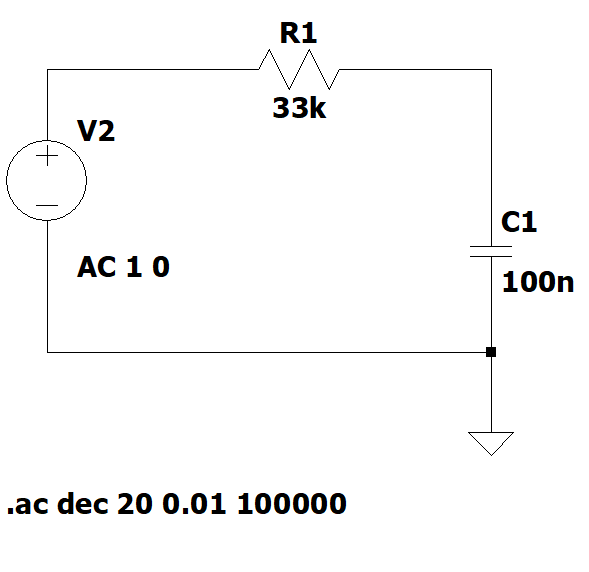
\includegraphics[width=\linewidth,height=0.46\textheight,keepaspectratio]{slides/img/ltspice_circuito_1.png}
    \end{column}
    \begin{column}{0.31\textwidth}
      \centering
      \textbf{Carga direta}

      \vspace{0.14cm}
      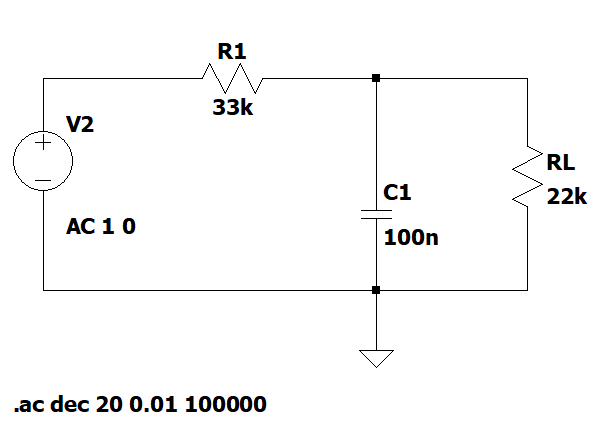
\includegraphics[width=\linewidth,height=0.46\textheight,keepaspectratio]{slides/img/ltspice_circuito_2.png}
    \end{column}
    \begin{column}{0.31\textwidth}
      \centering
      \textbf{Com buffer}

      \vspace{0.14cm}
      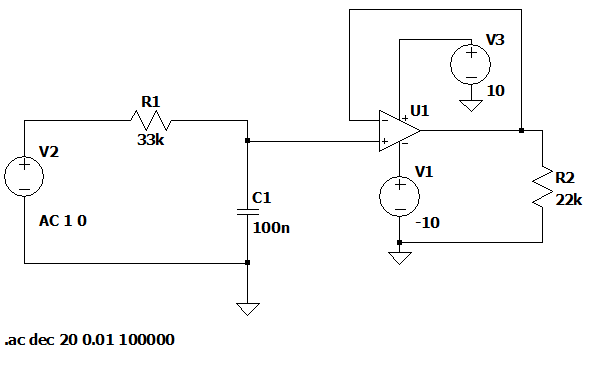
\includegraphics[width=\linewidth,height=0.46\textheight,keepaspectratio]{slides/img/ltspice_circuito_3.png}
    \end{column}
  \end{columns}

  \small
  \begin{block}{Configuração do projeto nominal}
    Entrada AC unitária; varredura de $0{,}01$ a $10^5\,\mathrm{Hz}$, com 20 pontos
    por década. Buffer alimentado em $\pm10\,\mathrm{V}$.
    As capturas utilizam $R=33\,\mathrm{k}\Omega$ e $R_L=22\,\mathrm{k}\Omega$.
  \end{block}
\end{frame}

\begin{frame}{Validação no LTspice: diagramas de Bode}
  \begin{columns}[T,onlytextwidth]
    \begin{column}{0.31\textwidth}
      \centering
      \textbf{Sem carga}

      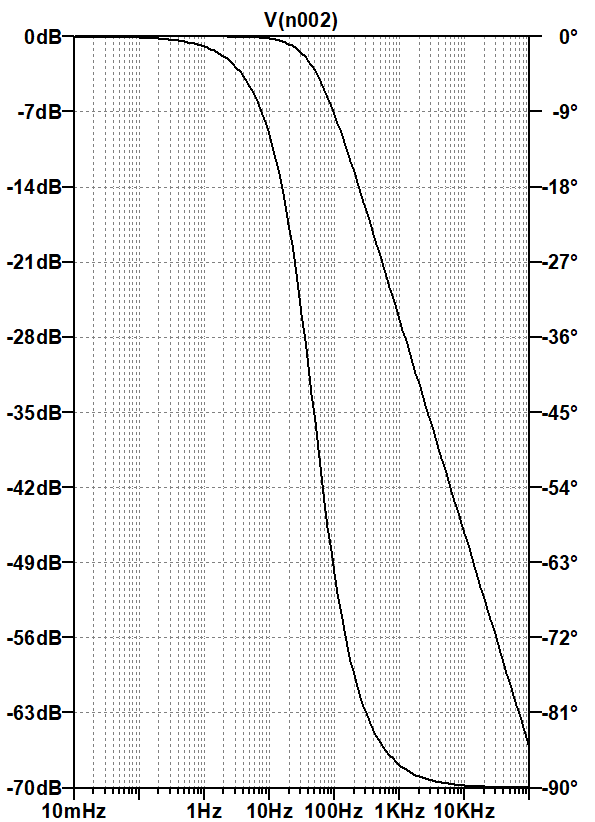
\includegraphics[height=0.52\textheight,width=\linewidth,keepaspectratio]{slides/img/ltspice_bode_1.png}

      \small Patamar próximo de $0\,\mathrm{dB}$.
    \end{column}
    \begin{column}{0.31\textwidth}
      \centering
      \textbf{Carga direta}

      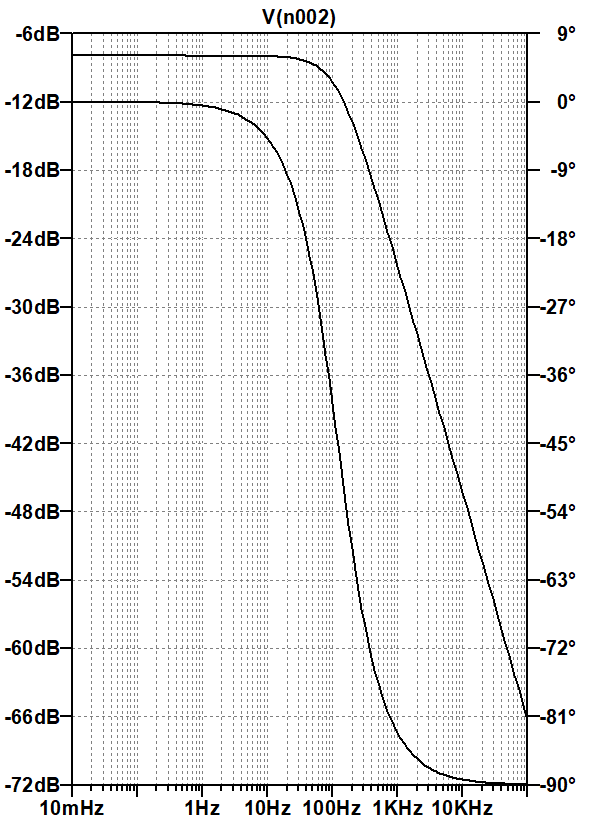
\includegraphics[height=0.52\textheight,width=\linewidth,keepaspectratio]{slides/img/ltspice_bode_2.png}

      \small Patamar atenuado e corte deslocado.
    \end{column}
    \begin{column}{0.31\textwidth}
      \centering
      \textbf{Com buffer}

      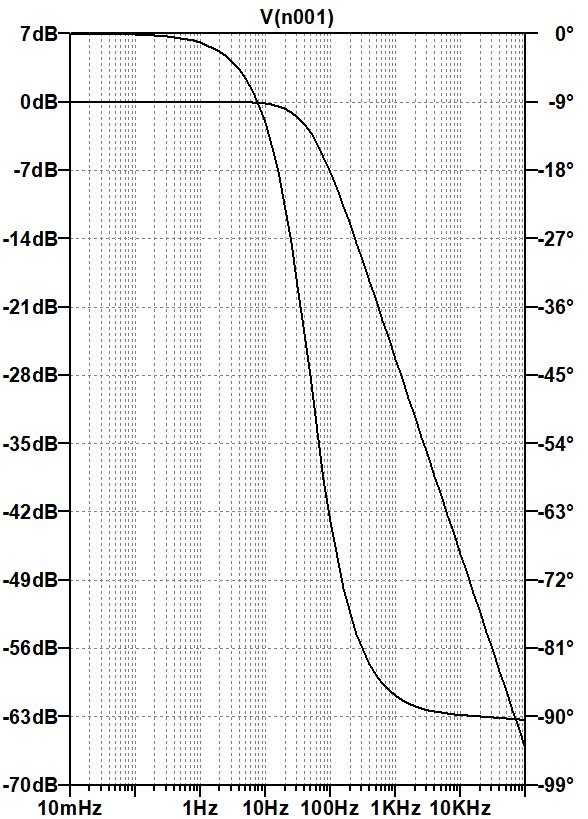
\includegraphics[height=0.52\textheight,width=\linewidth,keepaspectratio]{slides/img/ltspice_bode_3.png}

      \small Recuperação da resposta sem carga.
    \end{column}
  \end{columns}

  \vspace{0.10cm}
  \centering\scriptsize
  Capturas originais das simulações do projeto nominal.
  A comparação é qualitativa; magnitude e fase aparecem no mesmo painel.
\end{frame}

\begin{frame}{Montagens e componentes medidos}
  \small
  \begin{columns}[T,onlytextwidth]
    \begin{column}{0.31\textwidth}
      \centering
      \textbf{Circuito 1}

      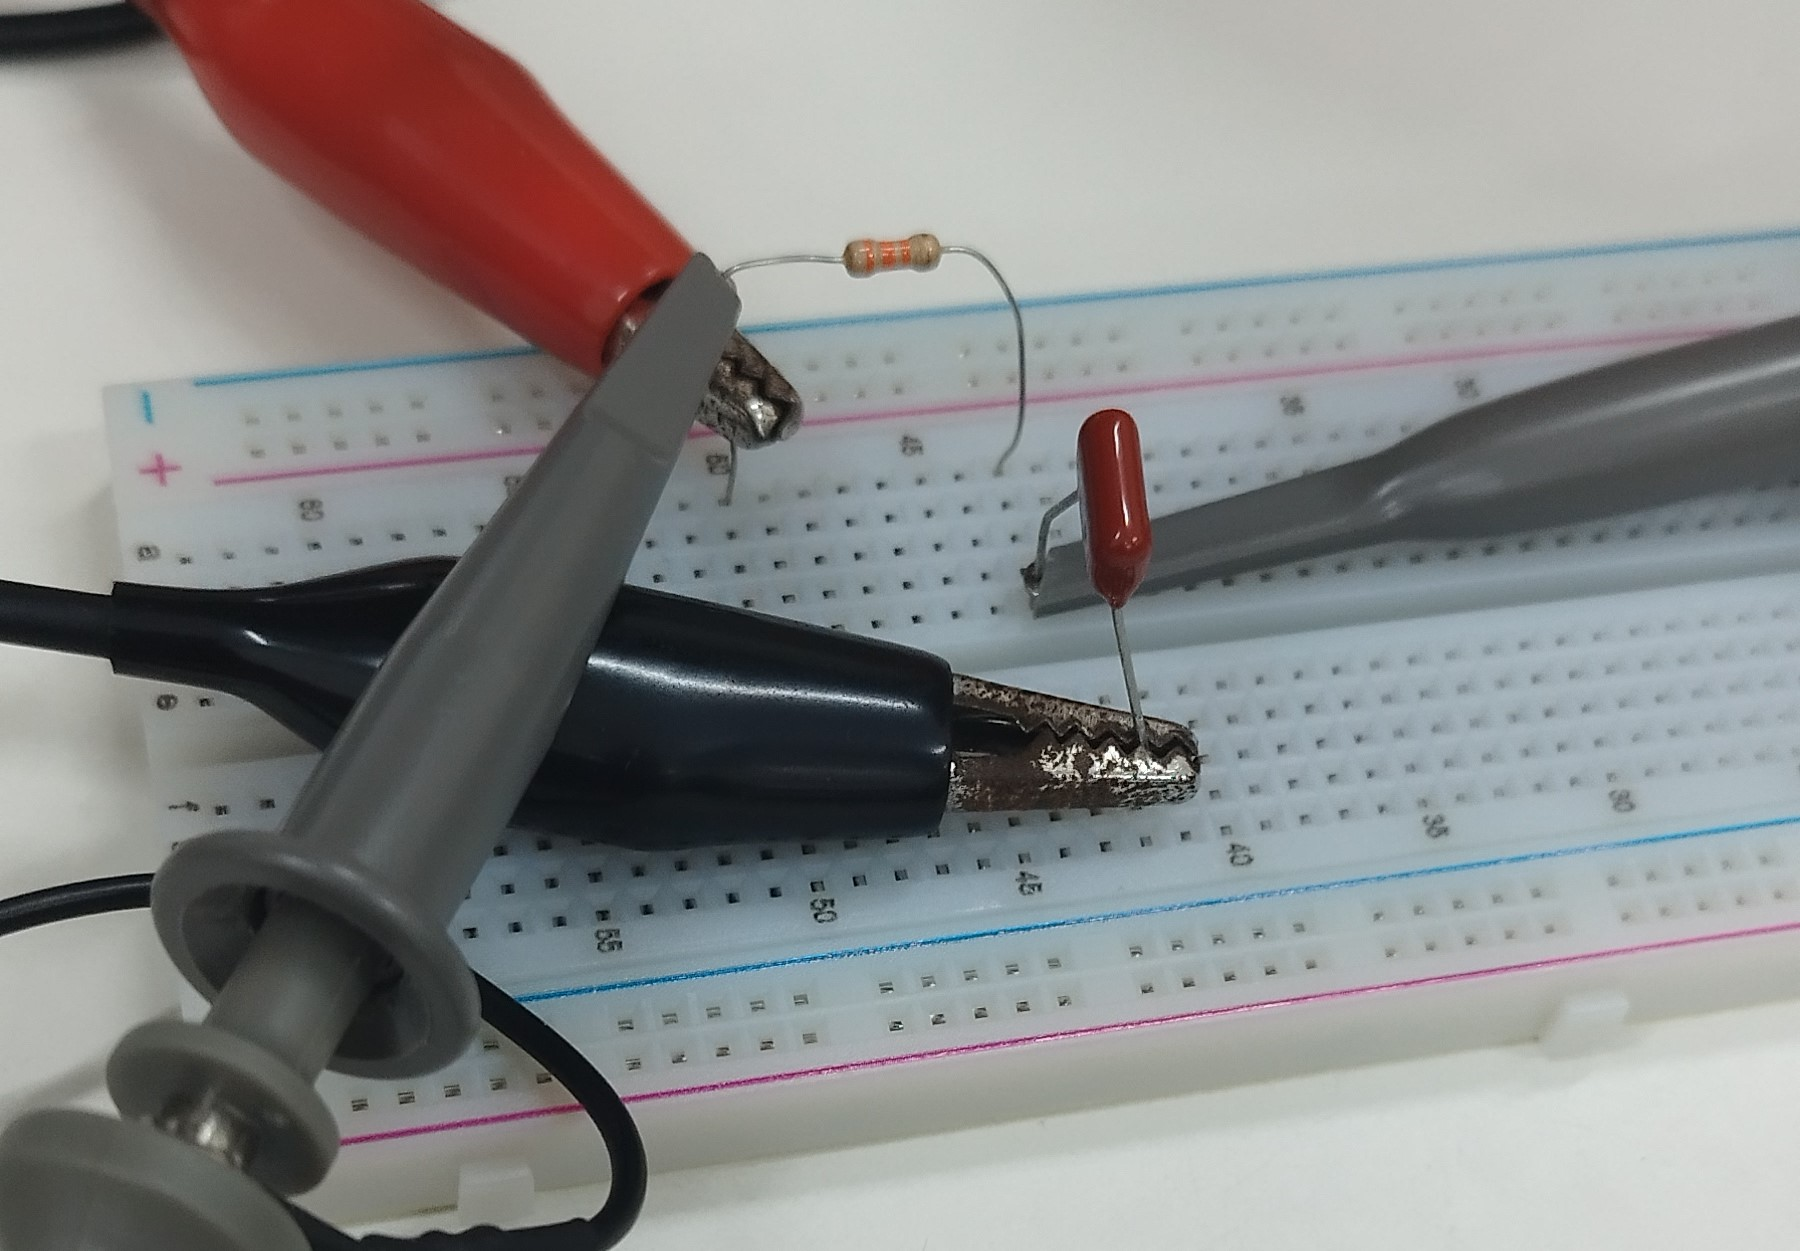
\includegraphics[width=\linewidth,height=0.24\textheight,keepaspectratio]{slides/img/protoboard_1.jpg}
    \end{column}
    \begin{column}{0.31\textwidth}
      \centering
      \textbf{Circuito 2}

      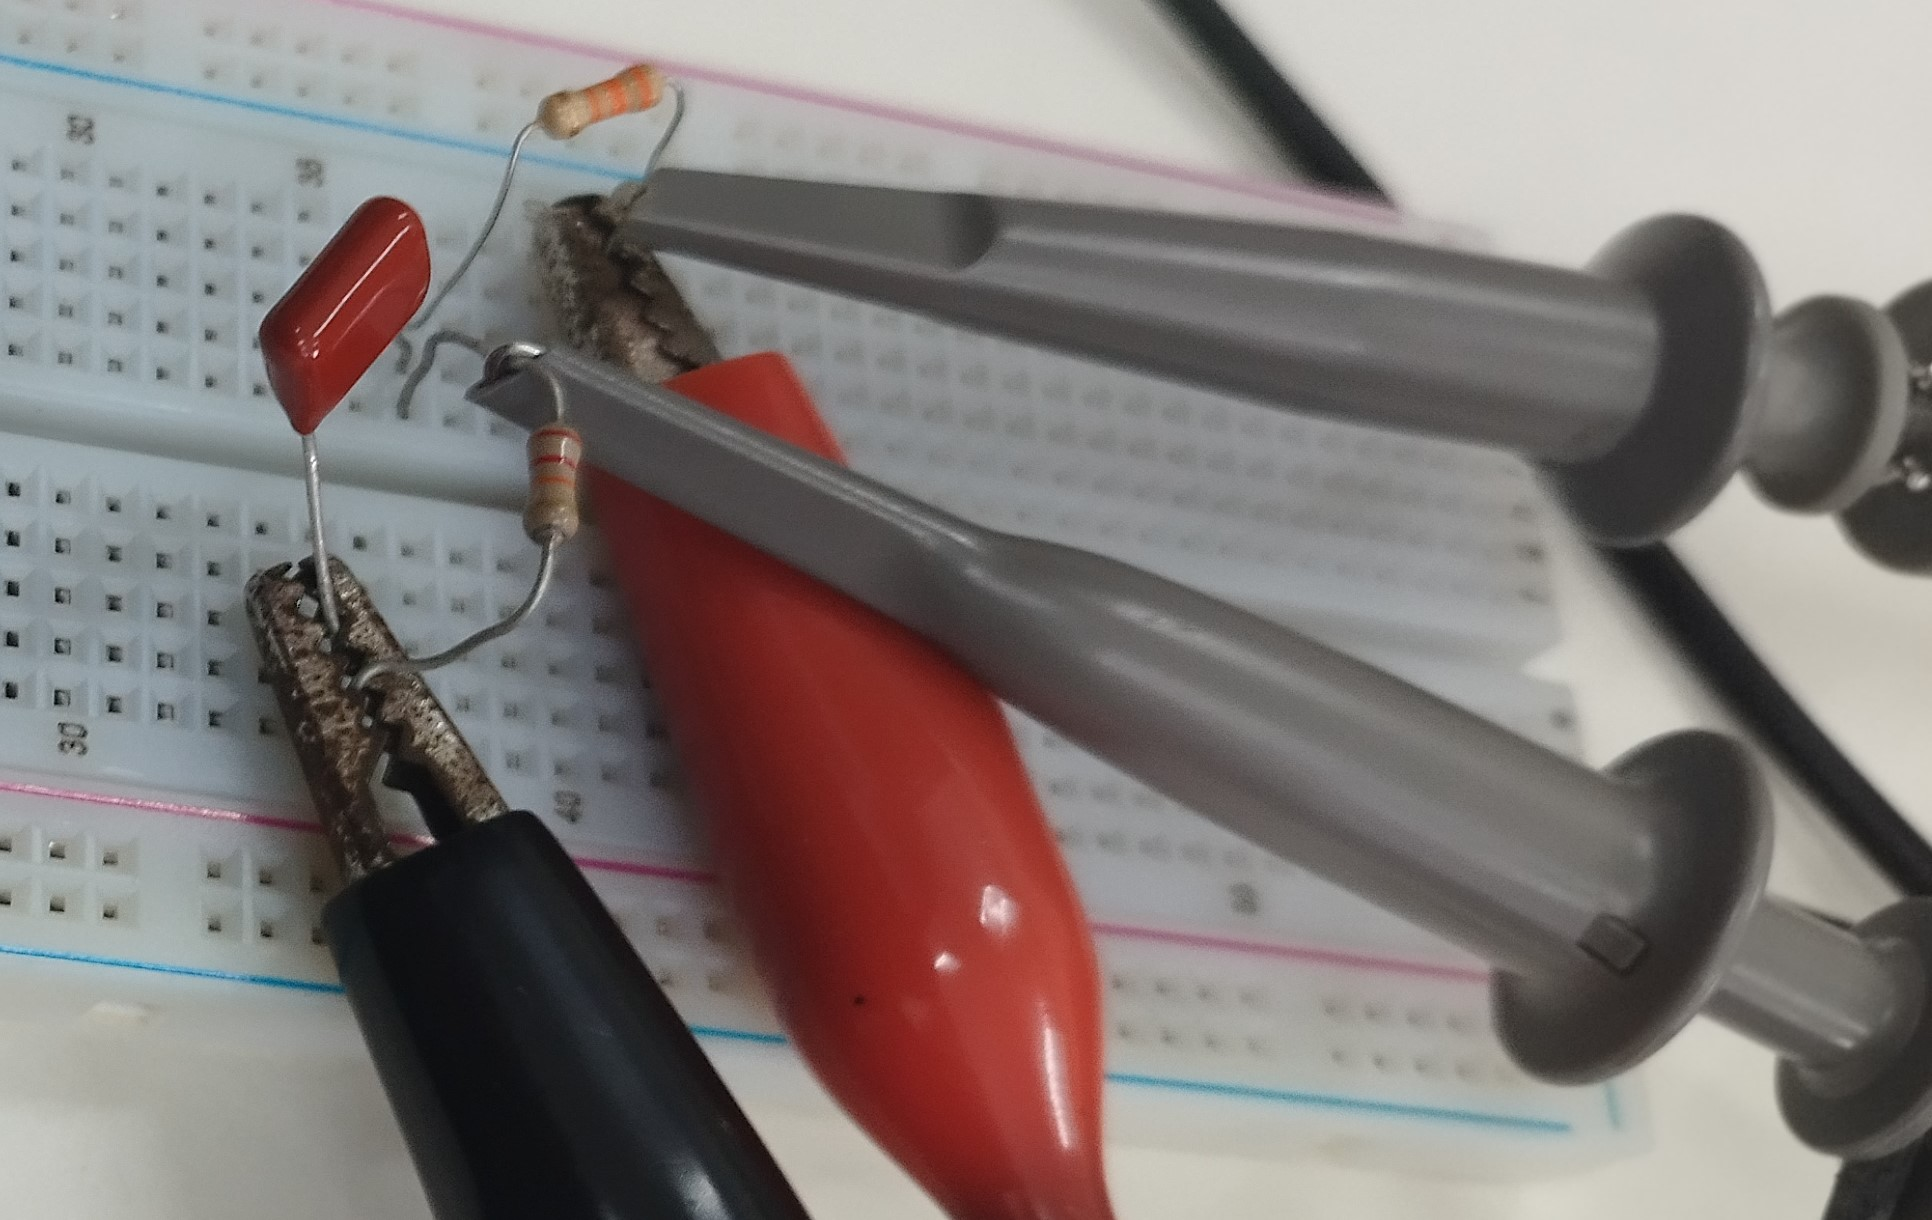
\includegraphics[width=\linewidth,height=0.24\textheight,keepaspectratio]{slides/img/protoboard_2.jpg}
    \end{column}
    \begin{column}{0.31\textwidth}
      \centering
      \textbf{Circuito 3}

      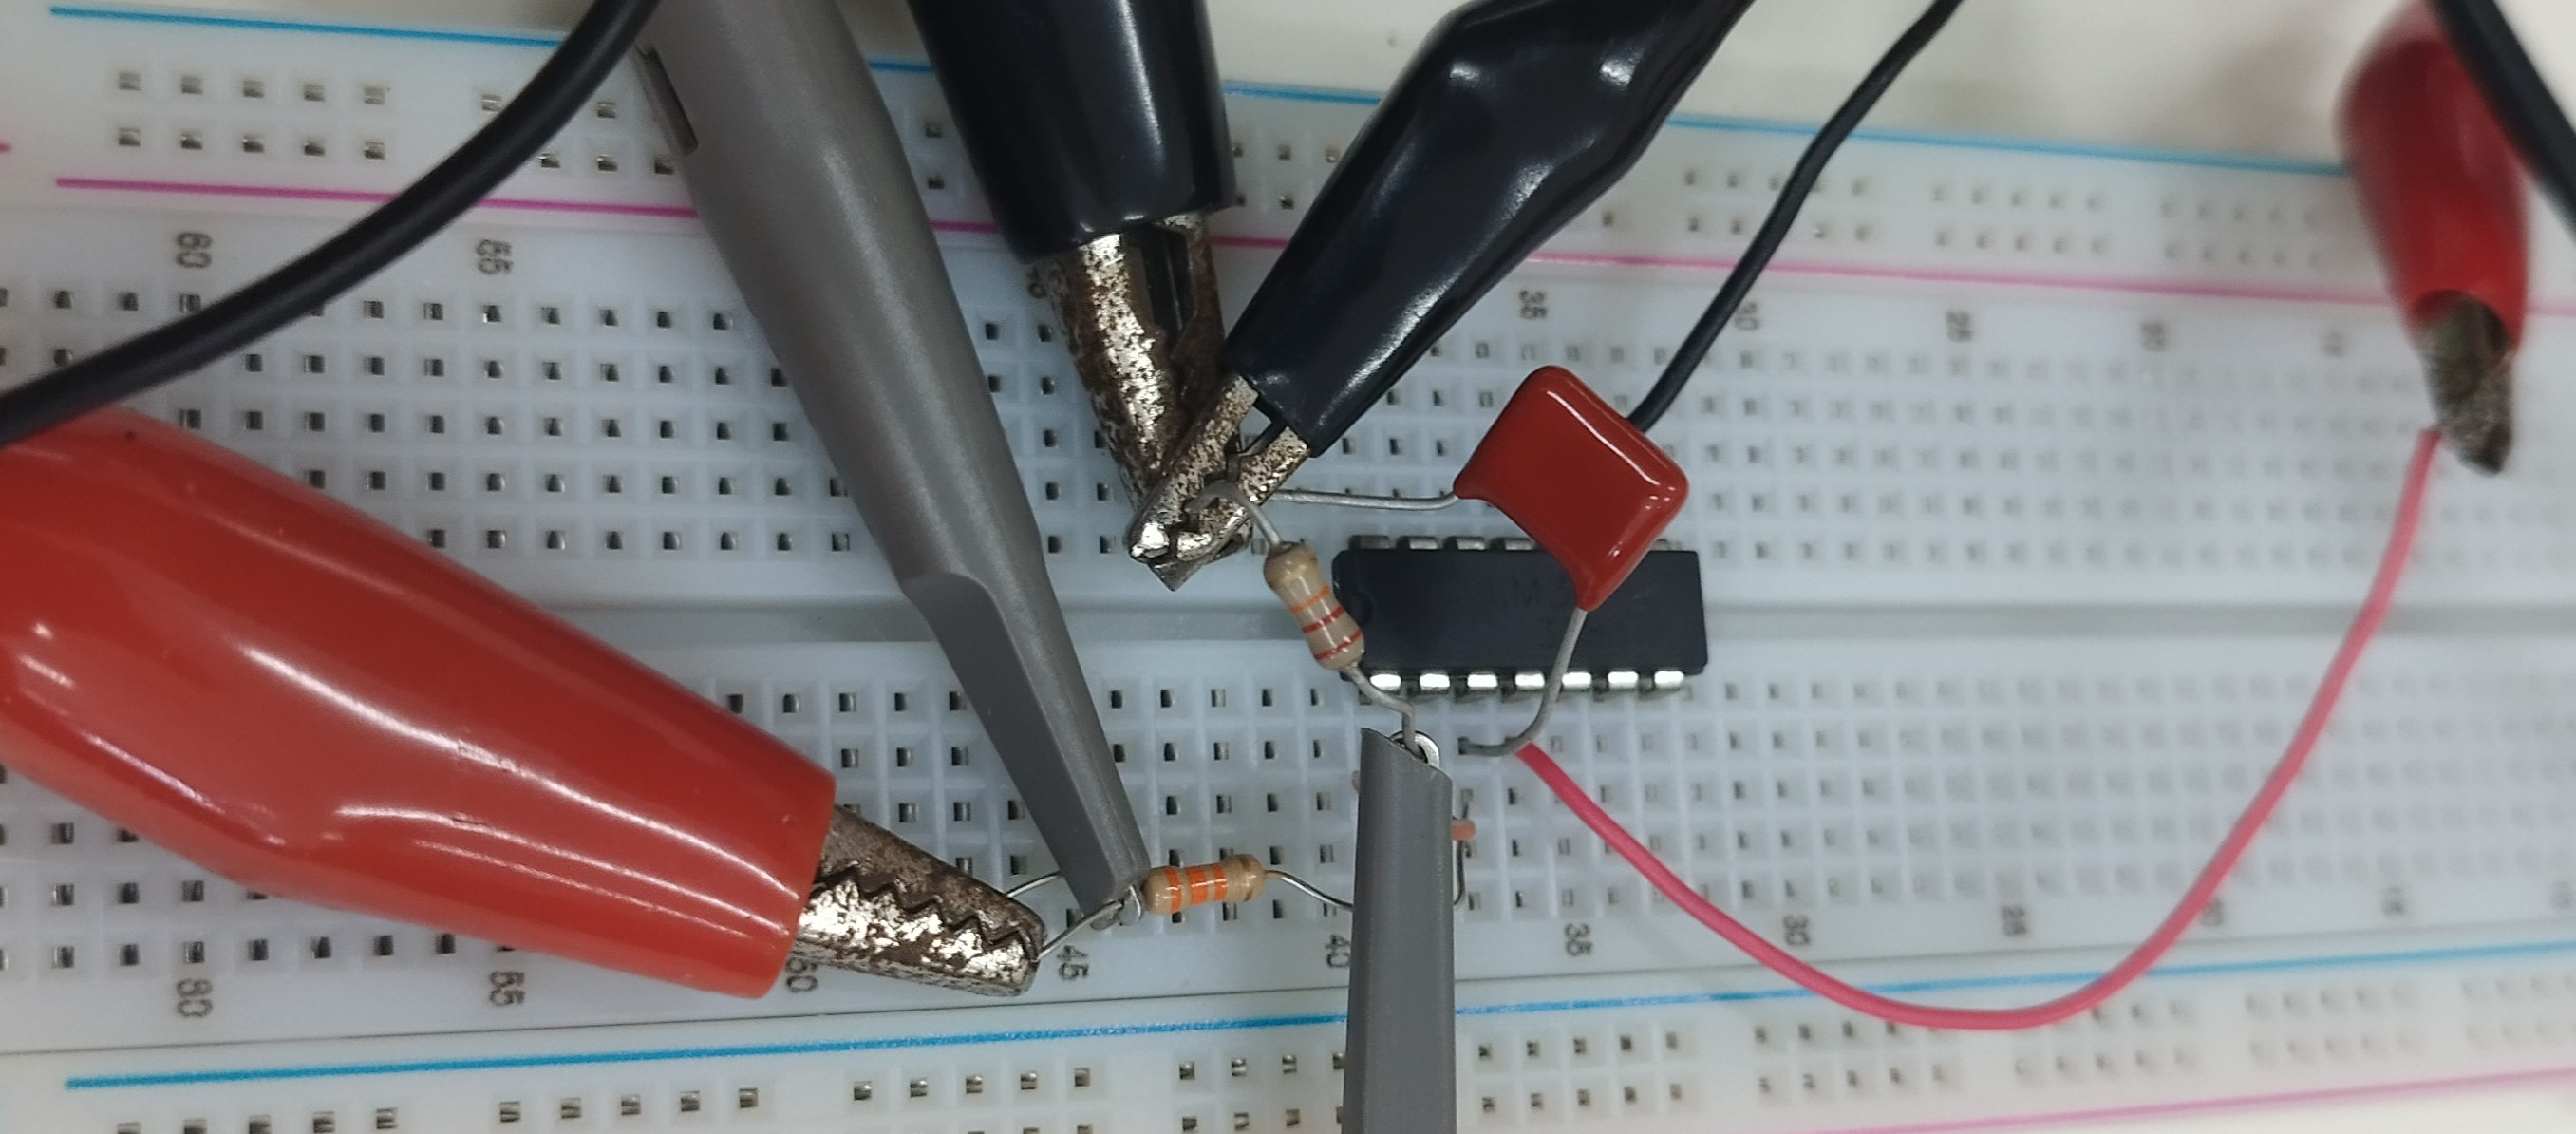
\includegraphics[width=\linewidth,height=0.24\textheight,keepaspectratio]{slides/img/protoboard_3.jpg}
    \end{column}
  \end{columns}

  \vspace{0.14cm}
  {\centering
    \renewcommand{\arraystretch}{1.0}
    \begin{tabular}{lccc}
      \toprule
      Circuito & $R$ ($\mathrm{k}\Omega$) & $C$ (nF) & $R_L$ ($\mathrm{k}\Omega$) \\
      \midrule
      1 -- sem carga & $21{,}841$ & $103{,}80$ & -- \\
      2 -- carga direta & $22{,}021$ & $110{,}90$ & $32{,}314$ \\
      3 -- buffer & $21{,}757$ & $106{,}28$ & $32{,}657$ \\
      \bottomrule
    \end{tabular}\par
  }

  \begin{alertblock}{Parâmetros da bancada}
    O conjunto medido difere do projeto de $50\,\mathrm{Hz}$.
    Cada modelo pós-laboratorial usa os componentes da respectiva montagem.
  \end{alertblock}
  \centering\scriptsize Registros de montagem das topologias; valores medidos usados nas comparações quantitativas.
\end{frame}

{
\pgfplotstableset{
  columns={f,vi,vo},
  columns/f/.style={column name={$f$ (Hz)},fixed,fixed zerofill,precision=2},
  columns/vi/.style={column name={$V_i$ (V)},fixed,fixed zerofill,precision=3},
  columns/vo/.style={column name={$V_o$ (V)},fixed,fixed zerofill,precision=3},
  /pgf/number format/use comma,
  every head row/.style={before row=\toprule,after row=\midrule},
  every last row/.style={after row=\bottomrule}
}
\begin{frame}{Amplitudes medidas nas três configurações}
  \scriptsize
  \setlength{\tabcolsep}{3pt}
  \renewcommand{\arraystretch}{1.0}
  \begin{columns}[T,onlytextwidth]
    \begin{column}{0.32\textwidth}
      \centering
      \textbf{1. Sem carga: $f_c=67\,\mathrm{Hz}$}

      \vspace{0.12cm}
      \pgfplotstabletypeset{slides/dados/medicoes_1.dat}
    \end{column}
    \begin{column}{0.32\textwidth}
      \centering
      \textbf{2. Carga: $f_c=121\,\mathrm{Hz}$}

      \vspace{0.12cm}
      \pgfplotstabletypeset{slides/dados/medicoes_2.dat}
    \end{column}
    \begin{column}{0.32\textwidth}
      \centering
      \textbf{3. Buffer: $f_c=69\,\mathrm{Hz}$}

      \vspace{0.12cm}
      \pgfplotstabletypeset{slides/dados/medicoes_3.dat}
    \end{column}
  \end{columns}

  \vspace{0.16cm}
  \centering
  Tensões pico a pico, convertidas para volts. A entrada é medida em cada ponto.
  Varredura de $0{,}02f_c$ a $20f_c$, conforme o roteiro.
\end{frame}
}


\section{Discussão}
\begin{frame}{Funções de transferência com componentes medidos}
  \small
  \begin{columns}[T,onlytextwidth]
    \begin{column}{0.31\textwidth}
      \begin{block}{1. Sem carga}
        \[
          H_1(s)\approx\frac{1}{1+0{,}00226710s}.
        \]
        \[
          \tau_1=2{,}2671\,\mathrm{ms}
        \]
        \[
          K_1=1
        \]
        \[
          f_{c1}\approx70{,}20\,\mathrm{Hz}.
        \]
      \end{block}
    \end{column}
    \begin{column}{0.31\textwidth}
      \begin{block}{2. Carga direta}
        \[
          H_2(s)\approx\frac{0{,}59472}{1+0{,}00145238s}.
        \]
        \[
          \tau_2=1{,}4524\,\mathrm{ms}
        \]
        \[
          K_2\approx0{,}59472
        \]
        \[
          f_{c2}\approx109{,}58\,\mathrm{Hz}.
        \]
      \end{block}
    \end{column}
    \begin{column}{0.31\textwidth}
      \begin{block}{3. Com buffer}
        \[
          H_3(s)\approx\frac{1}{1+0{,}00231233s}.
        \]
        \[
          \tau_3=2{,}3123\,\mathrm{ms}
        \]
        \[
          K_3=1
        \]
        \[
          f_{c3}\approx68{,}83\,\mathrm{Hz}.
        \]
      \end{block}
    \end{column}
  \end{columns}

  \vspace{0.12cm}
  \centering\scriptsize
  No circuito 2, $R\parallel R_L\approx13{,}0963\,\mathrm{k}\Omega$.
  As diferenças entre os cortes dos circuitos 1 e 3 decorrem dos componentes medidos.
\end{frame}

\begin{frame}{Comparação em bancada: filtro sem carga}
  \begin{columns}[c,onlytextwidth]
    \begin{column}{0.61\textwidth}
      \centering
      \begin{tikzpicture}
        \begin{loglogaxis}[
          grafico,height=0.55\textheight,xmin=0.5,xmax=3000,ymin=0.01,ymax=1.3,
          xlabel={Frequência (Hz)},ylabel={Magnitude $|H|$ (V/V)},legend pos=south west
        ]
          \addplot[very thick,RoxoPrincipal] table[x=f,y=modulo1]{slides/dados/resposta_ajustada.dat};
          \addlegendentry{Modelo com $R$, $C$ medidos}
          \addplot[only marks,mark=*,mark size=2pt,MalvaDestaque]
            table[x=f,y expr={\thisrow{vo}/\thisrow{vi}}]{slides/dados/medicoes_1.dat};
          \addlegendentry{Bancada}
        \end{loglogaxis}
      \end{tikzpicture}
    \end{column}
    \begin{column}{0.35\textwidth}
      \small
      \begin{block}{Ganho em baixa frequência}
        A $1\,\mathrm{Hz}$:
        \[
          \frac{469{,}1\,\mathrm{mV}}{483{,}2\,\mathrm{mV}}
          \approx0{,}971.
        \]
        Valor teórico: $K_1=1$.
      \end{block}
      \begin{alertblock}{Frequência de corte}
        Teoria: $70{,}20\,\mathrm{Hz}$.\\
        Registro: $67\,\mathrm{Hz}$.\\
        Diferença relativa: $4{,}56\%$.
      \end{alertblock}
    \end{column}
  \end{columns}
  \vspace{0.08cm}
  \centering\scriptsize Os pontos usam a razão $V_o/V_i$ das tensões medidas; a curva usa os componentes aferidos.
\end{frame}

\begin{frame}{Comparação em bancada: carga direta}
  \begin{columns}[c,onlytextwidth]
    \begin{column}{0.61\textwidth}
      \centering
      \begin{tikzpicture}
        \begin{loglogaxis}[
          grafico,height=0.55\textheight,xmin=0.5,xmax=3000,ymin=0.01,ymax=1.3,
          xlabel={Frequência (Hz)},ylabel={Magnitude $|H|$ (V/V)},legend pos=south west
        ]
          \addplot[very thick,RoxoPrincipal] table[x=f,y=modulo2]{slides/dados/resposta_ajustada.dat};
          \addlegendentry{Modelo com $R$, $C$, $R_L$ medidos}
          \addplot[only marks,mark=*,mark size=2pt,MalvaDestaque]
            table[x=f,y expr={\thisrow{vo}/\thisrow{vi}}]{slides/dados/medicoes_2.dat};
          \addlegendentry{Bancada}
        \end{loglogaxis}
      \end{tikzpicture}
    \end{column}
    \begin{column}{0.35\textwidth}
      \small
      \begin{block}{Atenuação de passagem}
        Medição em $2{,}42\,\mathrm{Hz}$:
        \[
          K_{\mathrm{med}}\approx\frac{0{,}460}{1{,}140}
          \approx0{,}404.
        \]
        Teoria: $K_2\approx0{,}595$.
      \end{block}
      \begin{alertblock}{Corte relativo ao patamar}
        $K_{\mathrm{med}}/\sqrt{2}\approx0{,}285$.\\
        Em $121\,\mathrm{Hz}$:
        \[
          |H|=\frac{1{,}470}{5{,}100}\approx0{,}288.
        \]
      \end{alertblock}
    \end{column}
  \end{columns}
  \vspace{0.08cm}
  \centering\scriptsize Corte teórico: $109{,}58\,\mathrm{Hz}$. A divergência do ganho de passagem requer análise das condições de medição.
\end{frame}

\begin{frame}{Comparação em bancada: isolamento com buffer}
  \begin{columns}[c,onlytextwidth]
    \begin{column}{0.61\textwidth}
      \centering
      \begin{tikzpicture}
        \begin{loglogaxis}[
          grafico,height=0.55\textheight,xmin=0.5,xmax=3000,ymin=0.01,ymax=1.3,
          xlabel={Frequência (Hz)},ylabel={Magnitude $|H|$ (V/V)},legend pos=south west
        ]
          \addplot[very thick,RoxoPrincipal] table[x=f,y=modulo3]{slides/dados/resposta_ajustada.dat};
          \addlegendentry{Modelo com $R$, $C$ medidos}
          \addplot[only marks,mark=*,mark size=2pt,MalvaDestaque]
            table[x=f,y expr={\thisrow{vo}/\thisrow{vi}}]{slides/dados/medicoes_3.dat};
          \addlegendentry{Bancada}
        \end{loglogaxis}
      \end{tikzpicture}
    \end{column}
    \begin{column}{0.35\textwidth}
      \small
      \begin{block}{Ganho restaurado}
        A $1\,\mathrm{Hz}$:
        \[
          \frac{480\,\mathrm{mV}}{500\,\mathrm{mV}}=0{,}960.
        \]
        Valor ideal: $K_3=1$.
      \end{block}
      \begin{alertblock}{Frequência de corte}
        Teoria: $68{,}83\,\mathrm{Hz}$.\\
        Registro: $69\,\mathrm{Hz}$.\\
        Diferença relativa: $0{,}25\%$.
      \end{alertblock}
    \end{column}
  \end{columns}
  \vspace{0.08cm}
  \centering\scriptsize O buffer recupera o comportamento próximo do filtro sem carga, apesar de $R_L$ permanecer conectada à saída.
\end{frame}

\begin{frame}{Síntese dos resultados e limites da comparação}
  \small
  {\centering
    \setlength{\tabcolsep}{5pt}
    \renewcommand{\arraystretch}{0.95}
    \begin{tabular}{lrrrrrr}
      \toprule
      & \multicolumn{3}{c}{Frequência de corte (Hz)} & \multicolumn{3}{c}{Ganho de passagem (V/V)} \\
      \cmidrule(lr){2-4}\cmidrule(lr){5-7}
      Circuito & Teoria & Medido & Erro & Teoria & Medido & Erro \\
      \midrule
      Sem carga & $70{,}20$ & $67$ & $4{,}56\%$ & $1{,}000$ & $0{,}971$ & $2{,}92\%$ \\
      Carga direta & $109{,}58$ & $121$ & $10{,}42\%$ & $0{,}595$ & $0{,}404$ & $32{,}15\%$ \\
      Buffer & $68{,}83$ & $69$ & $0{,}25\%$ & $1{,}000$ & $0{,}960$ & $4{,}00\%$ \\
      \bottomrule
    \end{tabular}\par
  }

  \centering\scriptsize Erros relativos à teoria com componentes medidos, calculados antes do arredondamento.
  \par\small
  \begin{columns}[T,onlytextwidth]
    \begin{column}{0.48\textwidth}
      \begin{block}{Resultados sustentados}
        \begin{itemize}
          \item A carga direta reduz o ganho e desloca o corte.
          \item O buffer aproxima a resposta daquela sem carga.
          \item A tensão de entrada medida permite comparar toda a varredura.
        \end{itemize}
      \end{block}
    \end{column}
    \begin{column}{0.48\textwidth}
      \begin{alertblock}{Limites da interpretação}
        \begin{itemize}
          \item O ganho do circuito 2 diverge do modelo em $32{,}15\%$.
          \item Convém conferir componentes, conexões e referência de entrada.
          \item Os dados não isolam uma causa para esse desvio.
        \end{itemize}
      \end{alertblock}
    \end{column}
  \end{columns}
\end{frame}


\section{Conclusão}
\begin{frame}{Conclusões}
  \begin{itemize}
    \item O filtro RC é um passa-baixa de primeira ordem, com
      $H_1(s)=1/(1+sRC)$ e ganho DC unitário.
    \item Para $50\,\mathrm{Hz}$ e $100\,\mathrm{nF}$, o projeto resulta em
      $R\approx31{,}83\,\mathrm{k}\Omega$; com $33\,\mathrm{k}\Omega$, o corte é $48{,}23\,\mathrm{Hz}$.
    \item A carga direta cria um divisor resistivo e altera a constante de tempo para
      $(R\parallel R_L)C$.
    \item O buffer ideal restaura $H_3(s)=H_1(s)$ ao isolar a carga do nó capacitivo.
    \item Na bancada, os cortes registrados foram $67$, $121$ e $69\,\mathrm{Hz}$;
      com buffer, o ganho de baixa frequência foi $0{,}960$.
  \end{itemize}

  \begin{alertblock}{Síntese da prática}
    O comportamento de um filtro depende de sua carga.
    O seguidor de tensão permite preservar a resposta do estágio RC,
    respeitadas as limitações do amplificador real.
  \end{alertblock}
\end{frame}


\section{Referências}
\begingroup
\setbeamertemplate{bibliography item}[text]
\setbeamercolor{bibliography item}{fg=MalvaDestaque}
\setbeamercolor{bibliography entry author}{fg=RoxoPrincipal}
\setbeamercolor{bibliography entry title}{fg=CinzaTexto}
\setbeamercolor{bibliography entry location}{fg=RoxoSecundario}
\setbeamerfont{bibliography entry author}{series=\bfseries}
\setbeamertemplate{bibliography entry title}{\hspace{0.35em}}
\setbeamertemplate{bibliography entry location}{\hspace{0.35em}}
\setbeamertemplate{bibliography entry note}{\hspace{0.35em}}

\begin{frame}[t]{Referências bibliográficas}
  \vspace{0.04cm}
  \fontsize{8.2}{9.3}\selectfont
  \nocite{*}
  \bibliographystyle{plain}
  \bibliography{referencias}
\end{frame}
\endgroup


{
\setbeamercolor{background canvas}{bg=RoxoPrincipal}
\setbeamertemplate{footline}{}
\begin{frame}[plain]
  \begin{center}
    \vfill
    \marcaInstitucional{1.25cm}\par
    \vspace{0.55cm}
    {\color{white}\Huge\bfseries OBRIGADO}\par
    \vspace{0.4cm}
    {\color{MalvaDestaque}\rule{0.22\textwidth}{2pt}}\par
    \vspace{0.55cm}
    {\usebeamerfont{author}\color{white}\insertauthor\par}
    \vspace{0.18cm}
    {\usebeamerfont{institute}\color{white!84}\insertinstitute\par}
    \vspace{0.32cm}
    {\color{MalvaDestaque}\small\bfseries\portfolio\par}
    \vfill
  \end{center}
\end{frame}
}


\end{document}
